% =====================================================================
%  Cinema Seat Reservation
%  DDD, TDD and Clean Architecture - Group Coursework Report
%  Compile with: pdflatex coursework_report.tex  (run twice for TOC/links)
% =====================================================================
\documentclass[11pt,a4paper]{article}

% ---------- encoding & fonts ----------
\usepackage[utf8]{inputenc}
\usepackage[T1]{fontenc}
\usepackage{lmodern}
\usepackage{microtype}

% ---------- layout ----------
\usepackage[a4paper,margin=2.5cm,top=3cm,bottom=3cm]{geometry}
\usepackage{parskip}
\usepackage{setspace}
\setstretch{1.15}

% ---------- structure & headers ----------
\usepackage{fancyhdr}
\usepackage{titlesec}

% ---------- tables ----------
\usepackage{booktabs}
\usepackage{tabularx}
\usepackage{longtable}
\usepackage{array}
\usepackage{multirow}
\usepackage{ragged2e}

% ---------- colour ----------
\usepackage[table]{xcolor}
\definecolor{primary}{RGB}{0,51,102}
\definecolor{accent}{RGB}{0,102,153}
\definecolor{codebg}{RGB}{245,246,248}
\definecolor{codekeyword}{RGB}{0,51,102}
\definecolor{codestring}{RGB}{163,47,21}
\definecolor{codecomment}{RGB}{99,110,124}

% ---------- code listings ----------
\usepackage{listings}

\lstdefinestyle{python}{%
  language=Python,
  basicstyle=\ttfamily\footnotesize,
  keywordstyle=\color{codekeyword}\bfseries,
  commentstyle=\color{codecomment}\itshape,
  stringstyle=\color{codestring},
  showstringspaces=false,
  numbers=left,
  numberstyle=\tiny\color{gray},
  numbersep=8pt,
  frame=single,
  rulecolor=\color{gray!40},
  backgroundcolor=\color{codebg},
  breaklines=true,
  columns=fullflexible,
  tabsize=4,
  keepspaces=true,
  aboveskip=0.8em,
  belowskip=0.8em,
}

\lstdefinestyle{shell}{%
  basicstyle=\ttfamily\footnotesize,
  frame=single,
  rulecolor=\color{gray!40},
  backgroundcolor=\color{codebg},
  breaklines=true,
  columns=fullflexible,
  aboveskip=0.8em,
  belowskip=0.8em,
}

% ---------- graphics ----------
\usepackage{graphicx}
\usepackage{tikz}
\usetikzlibrary{arrows.meta,positioning,shapes.geometric,calc}

% ---------- hyperlinks ----------
\usepackage[colorlinks=true,linkcolor=accent,urlcolor=accent,citecolor=accent]{hyperref}
\hypersetup{pdftitle={Cinema Seat Reservation - DDD, TDD and Clean Architecture}}

% ---------- section formatting ----------
\titleformat{\section}{\Large\bfseries\color{primary}}{\thesection.}{0.6em}{}
\titleformat{\subsection}{\large\bfseries\color{primary}}{\thesubsection.}{0.6em}{}
\titleformat{\subsubsection}{\normalsize\bfseries\color{accent}}{\thesubsubsection.}{0.6em}{}
\titleformat{\paragraph}{\normalsize\bfseries}{\theparagraph.}{0.6em}{}

% ---------- header / footer ----------
\pagestyle{fancy}
\fancyhf{}
\fancyhead[L]{\footnotesize\color{gray} Cinema Seat Reservation --- DDD, TDD and Clean Architecture}
\fancyhead[R]{\footnotesize\color{gray} Group Coursework}
\fancyfoot[C]{\thepage}
\renewcommand{\headrulewidth}{0.3pt}
\renewcommand{\footrulewidth}{0pt}

% ---------- handy macros ----------
\newcommand{\code}[1]{\texttt{#1}}
\newcommand{\component}[1]{\textbf{\code{#1}}}
\newcommand{\toarrow}{$\rightarrow$}

\begin{document}

% =====================================================================
%  TITLE PAGE
% =====================================================================
\begin{titlepage}
  \thispagestyle{empty}
  \begin{center}
    \vspace*{1.2cm}
    {\color{primary}\rule{\textwidth}{1.5pt}}\\[0.6cm]
    {\Huge\bfseries\color{primary} Cinema Seat Reservation}\\[0.5cm]
    {\Large Domain-Driven Design, Test-Driven Development and Clean Architecture}\\[0.4cm]
    {\color{primary}\rule{\textwidth}{1.5pt}}\\[1.2cm]

    {\large\bfseries Group Coursework Report}\\[1.2cm]

    {\large Department of Networks}\\
    {\large School of Computing and Informatics Technology}\\
    {\large Makerere University}
  \end{center}

  \vfill

  \begin{center}
    {\large\bfseries Group Members}
  \end{center}

  \begin{center}
    \begin{tabularx}{0.86\textwidth}{l@{\hspace{2.5em}}r@{\hspace{1em}}X}
      \toprule
      \textbf{Name} & \textbf{Reg. No.} & \textbf{Role} \\
      \midrule
      BYAMUGISHA ANTHONY & 24/U/0360 & Domain Lead \\
      AKELLO BEATRICE & 24/U/25856/EVE & Domain Model Lead \\
      NDAWULA HABIBAH & 24/U/10049/EVE & Architecture Lead \\
      MENHYA JOSHUA KIBEDI & 24/U/06798/EVE & Integration Lead \\
      All members (shared) & --- & Testing \\
      \bottomrule
    \end{tabularx}
  \end{center}

  \vspace{1.4cm}

  \begin{center}
    {\large\bfseries Instructor: Kasozi W. Vincent}
  \end{center}

  \vfill

  \begin{center}
    {\itshape Academic Year 2026}\\
    {\large October 2026}
  \end{center}
\end{titlepage}

% =====================================================================
%  TABLE OF CONTENTS
% =====================================================================
\tableofcontents
\clearpage

% =====================================================================
%  1. INTRODUCTION
% =====================================================================
\section{Introduction}

\subsection{Problem Statement}

Cinema customers, such as anime lovers, need to reserve a specific seat for a
particular movie show, and the same seat must never be allocated to more than
one reservation for that show. The system must therefore coordinate reservation
confirmation with the seat inventory of the specific show, while preserving
valid reservation states and seat-allocation rules.

This coursework applies three practices to that problem: \textbf{Domain-Driven
Design} (DDD), \textbf{Test-Driven Development} (TDD) and \textbf{Clean
Architecture}. The approach mirrors how a real DDD project would be structured:
six explicit business rules drive a small domain model, the model is organised
into four clean layers, and the important behaviour is verified with automated
tests written test-first.

The implementation is deliberately small. It contains exactly two connected use
cases that communicate through one domain event:
\begin{enumerate}
  \item \textbf{Use case 1 --- Confirm a Seat Reservation} (the main use case).
  \item \textbf{Use case 2 --- Reserve the Seat in the Show} (a follow-up use
        case requested by the domain event that use case 1 raises).
\end{enumerate}

\subsection{Scope}

\begin{itemize}
  \item Confirm an existing seat reservation (use case 1).
  \item Reserve the corresponding seat in the show after confirmation (use
        case 2).
  \item Validate cinema seat numbers.
  \item Check eligibility for confirmation: the show must not have started, and
        the customer must hold fewer than four confirmed seats for that show.
  \item Enforce valid reservation state transitions (PENDING only).
  \item Maintain a seat inventory for each show and prevent double allocation.
  \item Raise and handle the \code{ReservationConfirmed} domain event that
        connects the two use cases.
  \item Work with pre-loaded PENDING reservations and shows stored in
        in-memory repositories, and return a success or failure result.
\end{itemize}

\subsection{Exclusions (Out of Scope)}

The following are explicitly out of scope: payment processing,
authentication, ticket pricing and tiers, temporary seat holds, refunds and
cancellations, ticket printing, movie recommendations, e-mail/SMS
notifications, venue-map design, production concurrency and locking, a
production database, a web or mobile interface, deployment, microservices and
message brokers, and the creation of reservations and shows. Reservations and
shows are loaded from in-memory repositories.

\subsection{Key Domain Terms}

\begin{description}
  \item[Reservation] A customer's request to obtain a particular seat for a
        particular show. It starts as \code{PENDING} and may become
        \code{CONFIRMED}.
  \item[Show] One scheduled screening of a movie, with its own start time and
        seat inventory.
  \item[ShowSeat] A specific seat within a specific show whose availability is
        managed independently of the same physical seat in other shows.
  \item[SeatNumber] A validated seat identifier such as \code{A10}.
  \item[PENDING] A reservation that exists but has not yet completed
        confirmation.
  \item[CONFIRMED] A reservation that has passed the confirmation rules and
        whose seat has been allocated in the show.
  \item[AVAILABLE] A \code{ShowSeat} that is currently available for
        allocation.
  \item[RESERVED] A \code{ShowSeat} that has already been allocated to a
        reservation.
  \item[ReservationConfirmed] The domain event raised when a reservation
        becomes \code{CONFIRMED}; it requests seat allocation in the show.
\end{description}

% =====================================================================
%  2. BUSINESS RULES
% =====================================================================
\section{Business Rules BR1--BR6}

Exactly six business rules are defined. Each rule corresponds to one of the six
required rule types, and each rule explicitly states the component responsible
for enforcing it and the outcome when it is violated. Table~\ref{tab:rules}
summarises all six rules; Sections~\ref{sec:domain-model} and
\ref{sec:architecture} show how each one is implemented.

\begin{table}[h]
  \centering
  \scriptsize
  \begin{tabularx}{\textwidth}{@{}c c X X X@{}}%
    \toprule
    \textbf{BR} & \textbf{Rule type} & \textbf{Rule statement} &
    \textbf{Responsible component} & \textbf{Violation outcome} \\
    \midrule
    BR1 & Value rule &
      A \code{SeatNumber} is valid only when it contains one uppercase row
      letter A--Z followed by a seat position 1--50. &
      Value Object \code{SeatNumber} & Reject creation with
      \code{InvalidSeatNumberError}; no entity is built. \\
    BR2 & Identity/state rule &
      A \code{Reservation} starts in \code{PENDING} and may transition to
      \code{CONFIRMED} only from \code{PENDING}. &
      Entity / Aggregate Root \code{Reservation} & Reject with
      \code{InvalidReservationStateError}; state remains unchanged. \\
    BR3 & Invariant rule &
      Within one \code{Show}, a \code{ShowSeat} may be allocated to at most one
      reservation. &
      Aggregate Root \code{Show} (child \code{ShowSeat}) & Reject with
      \code{SeatAlreadyReservedError}; the existing allocation is unchanged. \\
    BR4 & Cross-concept rule &
      A reservation is eligible for confirmation only when the show has not
      started and the customer has fewer than four confirmed seats for that
      show. &
      Domain Service \code{ReservationEligibilityService} & Reject with
      \code{ReservationNotEligibleError}; reservation stays \code{PENDING} and no
      event is raised. \\
    BR5 & Follow-up rule &
      When a reservation changes from \code{PENDING} to \code{CONFIRMED}, it
      raises a \code{ReservationConfirmed} domain event that requests the show
      to reserve that \code{SeatNumber}. &
      \code{Reservation} raises the event; \code{ReservationConfirmedHandler}
      requests the \code{Show}. & If the show rejects the allocation, neither
      aggregate is saved: the reservation stays \code{PENDING} and the seat is
      unchanged. \\
    BR6 & Lookup rule &
      A reservation must be retrieved from the repository before confirmation
      can proceed. &
      Application Service \code{ConfirmReservationService} using
      \code{ReservationRepository} & Return \code{ReservationNotFoundError}; no
      state changes and no event is raised. \\
    \bottomrule
  \end{tabularx}
  \caption{Summary of the six business rules, their responsible components and
    their violation outcomes.}
  \label{tab:rules}
\end{table}

\subsection{Discussion}

\textbf{BR1} is a value rule: it decides when a small domain value is valid.
Because seat numbers are interchangeable by value and never change identity,
the rule naturally lives in the value object's own constructor.

\textbf{BR2} is an identity and state rule: an identified object changes state.
The \code{Reservation} is an entity whose identity is its
\code{reservation\_id}, so the state machine lives on the entity itself and only
its own domain method \code{confirm()} can change the state.

\textbf{BR3} is an invariant rule: a rule that must always hold inside one
aggregate. The \code{Show} aggregate owns its collection of \code{ShowSeat}
child entities, and the invariant ``a seat may be allocated at most once'' is
enforced at the aggregate root, which is the only place that may change a seat.

\textbf{BR4} is a cross-concept rule: the decision needs information from more
than one concept --- the show's start time, the customer, and the customer's
existing confirmed seats in that show. It does not fit naturally on one entity,
so it is placed in a stateless \textbf{Domain Service}.

\textbf{BR5} is a follow-up rule: after something important happens in
Aggregate A (\code{Reservation} becomes \code{CONFIRMED}), another business
action must be requested in Aggregate B (\code{Show} reserves the seat). This
is the exact situation a \textbf{Domain Event} exists for.

\textbf{BR6} is a lookup rule: an existing aggregate must be retrieved before an
operation can continue. This is the responsibility of a \textbf{Repository}
driven by the \textbf{Application Service}, which is where use-case logic
belongs.

% =====================================================================
%  3. DOMAIN MODEL
% =====================================================================
\section{Domain Model}\label{sec:domain-model}

This section presents the DDD building blocks used in the domain and links each
one to the business rule it implements. Figure~\ref{fig:layers} (Section
\ref{sec:architecture}) also shows where each building block sits.

\subsection{Value Object: SeatNumber (BR1)}

A \code{SeatNumber} is a value object: it has no separate identity, it is
defined entirely by its row letter and position, and two seat numbers are equal
when their values are equal. It is immutable after creation and validates
itself during creation, which is where BR1 is enforced.

\begin{lstlisting}[style=python,caption={\code{SeatNumber}\ --- BR1 enforced in the value object's constructor.},label=lst:br1]
@dataclass(frozen=True)
class SeatNumber:
    value: str

    def __post_init__(self):
        if not isinstance(self.value, str):
            raise InvalidSeatNumberError("Seat number must be a string.")

        if not re.fullmatch(r"[A-Z][1-9][0-9]?", self.value):
            raise InvalidSeatNumberError(
                "Seat number must contain one row letter A-Z "
                "followed by a position from 1-50."
            )

        position = int(self.value[1:])
        if position < 1 or position > 50:
            raise InvalidSeatNumberError("Seat position must be between 1 and 50.")
\end{lstlisting}

\subsection{Entity / Aggregate Root: Reservation (BR2)}

A \code{Reservation} is identified by its \code{reservation\_id}. Identity is
stable while the state changes, which is what makes it an entity rather than a
value object. It is also the root of a small aggregate: it owns its own state
and its recorded domain events. Its \code{confirm()} method enforces BR2 ---
only a \code{PENDING} reservation may become \code{CONFIRMED} --- and records
the BR5 event in the process.

\begin{lstlisting}[style=python,caption={\code{Reservation.confirm()}\ --- BR2 state machine and BR5 event recording.},label=lst:br2]
def confirm(self):
    if self.status != ReservationStatus.PENDING:
        raise InvalidReservationStateError(
            "Only a PENDING reservation can be confirmed."
        )

    self.status = ReservationStatus.CONFIRMED
    self._events.append(
        ReservationConfirmed(
            reservation_id=self.reservation_id,
            customer_id=self.customer_id,
            show_id=self.show_id,
            seat_number=self.seat_number,
        )
    )
\end{lstlisting}

The events are collected with \code{pull\_events()}, which returns the recorded
events and clears the list, so the aggregate never leaks its internal list to
callers.

\subsection{Child Entity: ShowSeat}

A \code{ShowSeat} is a child entity inside the \code{Show} aggregate. Its
identity is its \code{seat\_number} within a specific show; two seats with the
same \code{SeatNumber} in different shows are different entities. Its state
changes from \code{AVAILABLE} to \code{RESERVED}, so it has a lifecycle, which
makes it an entity. It is never an aggregate root: seat availability only makes
sense inside a show, so \code{ShowSeat} cannot be modified independently. Its
\code{\_reserve()} method is aggregate-internal and may be called only by the
\code{Show} root.

\subsection{Aggregate B: Show (BR3)}

The \code{Show} aggregate owns its collection of \code{ShowSeat} child
entities. The aggregate root protects the BR3 invariant: within one show, a
seat may be allocated to at most one reservation. The guard in
\code{reserve\_seat()} is the only place a seat changes from available to
reserved, so the invariant cannot be bypassed from outside.

\begin{lstlisting}[style=python,caption={\code{Show.reserve\_seat()}\ --- BR3 invariant enforced at the aggregate root.},label=lst:br3]
def reserve_seat(self, seat_number, reservation_id, customer_id):
    """BR3 lives here. Refuse to overwrite an allocation that already exists."""
    seat = self.seat(seat_number)
    if seat.status == SeatStatus.RESERVED:
        raise SeatAlreadyReservedError(
            f"Seat {seat.seat_number.value} is already reserved "
            f"for show {self.show_id}."
        )
    seat._reserve(reservation_id, customer_id)
    return seat
\end{lstlisting}

The \code{Show} also owns the seat map, so it --- and not a repository ---
answers ``how many seats does this customer already hold in this show?''
through \code{confirmed\_seat\_count\_for()}, which gives the domain service
the information it needs for BR4 without touching persistence.

\subsection{Domain Service: ReservationEligibilityService (BR4)}

BR4 is a cross-concept rule. The decision requires the show's start time, the
customer, and the customer's confirmed seat count in that show. The rule spans
two aggregate concepts, so it is placed in a stateless domain service with no
collaborators; the service receives both aggregates as arguments and decides
the rule entirely inside the domain layer.

\begin{lstlisting}[style=python,caption={\code{ReservationEligibilityService}\ --- BR4 as a Domain Service.},label=lst:br4]
class ReservationEligibilityService:
    """Domain Service for BR4 (cross-concept rule, spans two aggregates)."""

    MAX_CONFIRMED_SEATS_PER_SHOW = 4

    def check_eligibility(self, reservation, show, current_time):
        """Raise ReservationNotEligibleError if BR4 rejects the reservation."""
        if current_time >= show.start_time:
            raise ReservationNotEligibleError(
                f"Show {show.show_id} has already started, so reservation "
                f"{reservation.reservation_id} cannot be confirmed."
            )

        held = show.confirmed_seat_count_for(reservation.customer_id)
        if held >= self.MAX_CONFIRMED_SEATS_PER_SHOW:
            raise ReservationNotEligibleError(
                f"Customer {reservation.customer_id} already holds {held} "
                f"seats for show {show.show_id}; the limit is "
                f"{self.MAX_CONFIRMED_SEATS_PER_SHOW}."
            )
\end{lstlisting}

\subsection{Factory Decision}

A factory is used for the \code{Show} only. \code{Show.create()} builds the
entire seat map --- ``every row exists and every seat starts AVAILABLE'' is a
construction rule rather than something each caller should assemble by hand.
No factory is used for \code{Reservation}: a reservation is fully described by
its constructor (\code{reservation\_id}, \code{customer\_id}, \code{show\_id},
\code{seat\_number}), so a factory would only add a name for it.

\subsection{Domain Event: ReservationConfirmed (BR5)}

When a \code{Reservation} is confirmed, it records a \code{ReservationConfirmed}
domain event carrying plain data only: \code{reservation\_id},
\code{customer\_id}, \code{show\_id} and \code{seat\_number}. It holds no
references to aggregates, so it is the only thing that crosses the boundary
between the two aggregates. Section \ref{sec:aggregate-communication} describes
the full flow.

\subsection{Repositories}

There is one repository abstraction per aggregate root used in the workflow.
The abstractions live in the \textbf{Application} layer (they are ports used by
use cases) and concrete in-memory implementations live in the
\textbf{Infrastructure} layer:

\begin{center}
  \begin{tabularx}{\textwidth}{@{}l l X@{}}
    \toprule
    \textbf{Abstraction (Application)} & \textbf{Implementation (Infrastructure)} & \textbf{Stores} \\
    \midrule
    \code{ReservationRepository}
      (\code{get\_by\_id}, \code{save}) &
    \code{InMemoryReservationRepository} &
    \code{Reservation} aggregates keyed by \code{reservation\_id}. \\
    \code{ShowRepository}
      (\code{get\_by\_id}, \code{save}) &
    \code{InMemoryShowRepository} &
    \code{Show} aggregates (with their seats) keyed by \code{show\_id}. \\
    \bottomrule
  \end{tabularx}
\end{center}

\code{ShowSeat} has no repository of its own: it lives inside the \code{Show}
aggregate and is only ever reached through the \code{Show} root. The in-memory
repositories store and return copies (implemented with \code{copy.deepcopy}),
like a database, so a rejected change is never saved. In-memory persistence
keeps the coursework small and makes the tests fast and repeatable.

% =====================================================================
%  4. CLEAN ARCHITECTURE
% =====================================================================
\section{Clean Architecture}\label{sec:architecture}

\subsection{The Four Layers}

The solution is organised into the four required areas: Domain, Application,
Infrastructure and Interface.

\begin{center}
  \resizebox{0.96\textwidth}{!}{%
  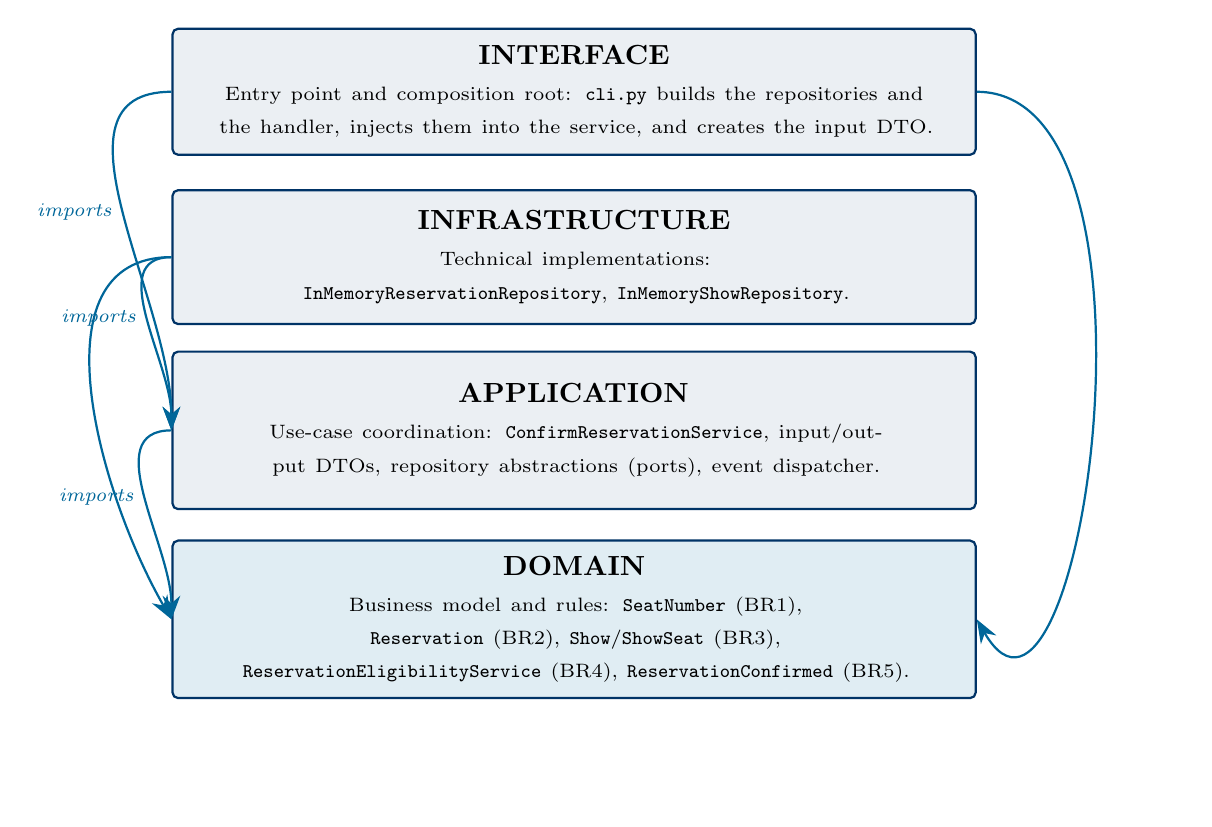
\begin{tikzpicture}[
      ylayer/.style={draw=primary, thick, fill=primary!8,
        minimum width=10.2cm, align=center, rounded corners=2pt},
      depends/.style={font=\scriptsize\itshape\color{gray}},
      imp/.style={-{Stealth[length=3mm]}, thick, color=accent},
    ]
    % Interface
    \node[ylayer, minimum height=1.6cm, text width=9.8cm]
      (interface) at (0,0) {%
        \textbf{INTERFACE}\\[1pt]
        \scriptsize Entry point and composition root: \code{cli.py} builds the
        repositories and the handler, injects them into the service, and
        creates the input DTO.};
    % Infrastructure
    \node[ylayer, minimum height=1.7cm, text width=9.8cm]
      (infra) at (0,-2.1) {%
        \textbf{INFRASTRUCTURE}\\[1pt]
        \scriptsize Technical implementations: \code{InMemoryReservationRepository},
        \code{InMemoryShowRepository}.};
    % Application
    \node[ylayer, minimum height=2.0cm, text width=9.8cm]
      (app) at (0,-4.3) {%
        \textbf{APPLICATION}\\[1pt]
        \scriptsize Use-case coordination: \code{ConfirmReservationService},
        input/output DTOs, repository abstractions (ports), event dispatcher.};
    % Domain
    \node[ylayer, minimum height=2.0cm, text width=9.8cm, fill=accent!12]
      (domain) at (0,-6.7) {%
        \textbf{DOMAIN}\\[1pt]
        \scriptsize Business model and rules: \code{SeatNumber} (BR1),
        \code{Reservation} (BR2), \code{Show}/\code{ShowSeat} (BR3),
        \code{ReservationEligibilityService} (BR4), \code{ReservationConfirmed} (BR5).};

    % Dependency arrows (pointing "inward" toward Domain)
    \draw[imp] (interface.west) to[out=180,in=90] node[depends,left]
      {imports} (app.west);
    \draw[imp] (app.west) to[out=180,in=90] node[depends,left]
      {imports} (domain.west);
    \draw[imp] (infra.west) to[out=180,in=90] node[depends,left]
      {imports} (app.west);
    \draw[imp] (infra.west) to[out=180,in=120] (domain.west);
    \draw[imp] (interface.east) to[out=0,in=300] (domain.east);
  \end{tikzpicture}}
\end{center}

\begin{itemize}
  \item \textbf{Domain} contains the entities, value objects, aggregate roots,
        domain service, domain events and business rules. It imports nothing
        outside itself.
  \item \textbf{Application} contains the application service, the DTOs, the
        repository abstractions and the event dispatcher. It depends only on
        the Domain layer.
  \item \textbf{Infrastructure} provides the in-memory repository
        implementations for the Application-layer ports.
  \item \textbf{Interface} is the minimal entry point: a CLI that acts as the
        composition root and wires concrete implementations into the service by
        dependency injection.
\end{itemize}

The source-code dependencies were verified with the provided checker, which
parses every import with the Python \code{ast} module:

\begin{lstlisting}[style=shell,caption={Result of \code{python scripts/check\_dependencies.py}.},label=lst:layers]
domain          -> (nothing)
application     -> domain
infrastructure  -> application, domain
interface       -> application, domain, infrastructure

OK: all imports point inward.
\end{lstlisting}

\subsection{Application Service and DTOs}

The main use case is implemented by \code{ConfirmReservationService}. It
\emph{coordinates} the workflow; it does not contain business rules. Its
responsibilities are: load the reservation (BR6), load the show, ask the domain
service for BR4, call \code{reservation.confirm()} (BR2), dispatch the BR5
event, and save only on success.

\begin{lstlisting}[style=python,caption={\code{ConfirmReservationService.execute()}\ --- use-case coordination with BR6 lookup.},label=lst:br6]
def execute(self, request):
    # BR6: the Reservation must already exist before confirmation proceeds.
    reservation = self._reservations.get_by_id(request.reservation_id)
    if reservation is None:
        raise ReservationNotFoundError(...)

    show = self._shows.get_by_id(reservation.show_id)
    if show is None:
        raise ShowNotFoundError(...)

    status_before = reservation.status

    try:
        # BR4 - decided by the Domain Service from the two aggregates.
        self._eligibility.check_eligibility(
            reservation=reservation, show=show,
            current_time=self._clock(),
        )
        reservation.confirm()                 # BR2, records BR5 event
        self._dispatcher.dispatch(reservation.pull_events())   # BR5 -> BR3
    except DomainError as error:
        # Nothing is saved, so the stored Reservation keeps its old status.
        return ConfirmReservationOutput(
            reservation_id=reservation.reservation_id,
            status=status_before.value, success=False, message=str(error),
        )

    self._reservations.save(reservation)
    return ConfirmReservationOutput(
        reservation_id=reservation.reservation_id,
        status=reservation.status.value, success=True,
        message="Reservation confirmed and seat reserved",
    )
\end{lstlisting}

The input and output DTOs carry data across the application boundary. They are
frozen dataclasses and contain no business logic.

\begin{center}
  \begin{tabularx}{\textwidth}{@{}l X@{}}
    \toprule
    \textbf{DTO} & \textbf{Contents} \\
    \midrule
    \code{ConfirmReservationInput} & \code{reservation\_id} --- identifies the
      reservation to confirm. \\
    \code{ConfirmReservationOutput} & \code{reservation\_id}, \code{status}
      (final stored status: \code{PENDING} or \code{CONFIRMED}), \code{success}
      (boolean), \code{message}. \\
    \bottomrule
  \end{tabularx}
\end{center}

\subsection{Dependency Injection}

The application service is supplied with everything it needs from outside its
class, through its constructor: the two repository abstractions, the domain
service, the event dispatcher, and an optional clock (fixed to a constant in
tests). The composition root is the Interface/CLI layer:

\begin{lstlisting}[style=python,caption={Composition root in \code{cli.py}\ --- dependencies injected from outside the service.},label=lst:di]
def build_service():
    reservations = InMemoryReservationRepository()
    shows = InMemoryShowRepository()

    dispatcher = EventDispatcher()
    dispatcher.register(ReservationConfirmed,
                        ReservationConfirmedHandler(shows).handle)

    service = ConfirmReservationService(
        reservation_repository=reservations,
        show_repository=shows,
        eligibility_service=ReservationEligibilityService(),
        event_dispatcher=dispatcher,
    )
    return service, reservations, shows
\end{lstlisting}

This keeps the application decoupled from infrastructure: the service depends
on abstractions, and the concrete in-memory implementations are chosen once, at
the entry point.

\subsection{Layer Supertype}

A \textbf{Layer Supertype} is a common base class for objects within a layer.
The project uses \code{DomainEvent} as the abstract base (supertype) of every
domain event. Because the dispatcher and any future subscriber program against
the \code{DomainEvent} abstraction rather than a growing list of concrete event
classes, new event types can be added without touching the dispatcher.
\code{DomainEvent} is a frozen ABC, keeping events immutable and guaranteeing
the layer supertype contract.

% =====================================================================
%  5. AGGREGATE COMMUNICATION
% =====================================================================
\section{Aggregate Communication (BR5)}\label{sec:aggregate-communication}

The two aggregates never hold a reference to each other. Communication across
the boundary happens only through the \code{ReservationConfirmed} domain event.
The complete flow is:

\begin{center}
  \resizebox{0.97\textwidth}{!}{%
  \begin{tikzpicture}[
      step/.style={draw=primary, thick, fill=primary!8, rounded corners=2pt,
        align=center, text width=2.7cm, minimum height=1.15cm},
      evt/.style={draw=accent, thick, fill=accent!12, rounded corners=2pt,
        align=center, text width=2.7cm, minimum height=1.15cm},
      capt/.style={font=\scriptsize\itshape\color{gray}, align=center, text width=2.7cm},
      arr/.style={-{Stealth[length=2.6mm]}, thick, color=accent},
    ]
    \node[step] (req) {Request\\ \scriptsize \code{ConfirmReservationInput}};
    \node[step, right=0.35cm of req] (svc) {Application\\ \scriptsize Service\\(BR6, BR4)};
    \node[step, right=0.35cm of svc] (rep) {Aggregate A\\ \scriptsize \code{Reservation.confirm()}\\(BR2, BR5)};
    \node[evt, right=0.35cm of rep] (ev) {Domain Event\\ \scriptsize \code{ReservationConfirmed}};
    \node[step, right=0.35cm of ev] (disp) {Event\\ \scriptsize Dispatcher};
    \node[step, right=0.35cm of disp] (hdl) {Handler\\ \scriptsize load-call-save};
    \node[step, right=0.35cm of hdl] (show) {Aggregate B\\ \scriptsize \code{Show.reserve\_seat()}\\(BR3)};

    \draw[arr] (req) -- (svc);
    \draw[arr] (svc) -- (rep);
    \draw[arr] (rep) -- (ev);
    \draw[arr] (ev) -- (disp);
    \draw[arr] (disp) -- (hdl);
    \draw[arr] (hdl) -- (show);

    \node[capt, below=0.15cm of req] {Input DTO};
    \node[capt, below=0.15cm of svc] {coordinates only};
    \node[capt, below=0.15cm of rep] {records the event};
    \node[capt, below=0.15cm of ev] {\code{reservation\_id}, \code{customer\_id},\\ \code{show\_id}, \code{seat\_number}};
    \node[capt, below=0.15cm of disp] {in-process routing};
    \node[capt, below=0.15cm of hdl] {load -- call -- save};
    \node[capt, below=0.15cm of show] {protects BR3 invariant};
  \end{tikzpicture}}
\end{center}

\noindent Step by step:

\begin{enumerate}
  \item The request arrives at the application service as a
        \code{ConfirmReservationInput} DTO.
  \item The service retrieves the reservation (BR6) and the show, then runs BR4
        through the domain service.
  \item Aggregate A --- \code{Reservation.confirm()} --- checks BR2 and changes
        the state from \code{PENDING} to \code{CONFIRMED}; it records the
        \code{ReservationConfirmed} event (BR5). \emph{What happened before the
        event was raised:} the reservation passed its eligibility rules and
        transitioned from \code{PENDING} to \code{CONFIRMED}.
  \item The service dispatches the collected events through the in-process
        \code{EventDispatcher}, which routes them to registered handlers by
        event type.
  \item The \emph{handler} (\code{ReservationConfirmedHandler}) receives the
        event and uses the \emph{load-call-save} pattern: it loads Aggregate B
        (\code{Show}) from its repository, calls \code{show.reserve\_seat(...)},
        and saves the show if the allocation succeeds.
  \item Aggregate B checks its own invariant (BR3): a \code{ShowSeat} may be
        allocated to at most one reservation. If the seat is already reserved,
        \code{SeatAlreadyReservedError} is raised, the handler does not save,
        and the application service returns a failure --- the reservation stays
        \code{PENDING} and the seat is unchanged (T8).
  \item Only if all domain rules pass does the service save the confirmed
        reservation.
\end{enumerate}

\emph{Key point:} the aggregates never modify each other directly. Aggregate A
records the event; the application dispatches it; the handler does load-call-save;
Aggregate B enforces its own rule before accepting the follow-up action.

% =====================================================================
%  6. TESTING AND TDD
% =====================================================================
\section{Testing and TDD}

\subsection{Test Suite T1--T8}

Eight automated tests with the identifiers T1--T8 cover the rules and the two
use cases. T1--T6 verify BR1--BR6 individually, T7 verifies the successful main
use case end-to-end, and T8 verifies the rejection path. In the submitted
project the T1--T6 identifiers each group a small number of parametrised test
functions (28 total), giving the rejection and boundary cases required by the
assignment.

\begin{center}
  \scriptsize
  \begin{tabularx}{\textwidth}{@{}l l X@{}}
    \toprule
    \textbf{Test} & \textbf{Rule / behaviour} & \textbf{Checks and expected results} \\
    \midrule
    \code{T1} & BR1 SeatNumber value rule &
      Valid and invalid seat numbers; boundary \code{A1}, \code{Z50} accepted;
      \code{A0} and \code{A51} rejected with \code{InvalidSeatNumberError}. \\
    \code{T2} & BR2 Reservation state rule &
      \code{PENDING} starts pending and can be confirmed; confirming an already
      \code{CONFIRMED} reservation raises \code{InvalidReservationStateError}. \\
    \code{T3} & BR3 Show invariant &
      Seats start \code{AVAILABLE}; a seat can be reserved once; reserving the
      same seat again raises \code{SeatAlreadyReservedError}; the same seat in
      a different show is independent; two different seats in one show can both
      be reserved. \\
    \code{T4} & BR4 eligibility & 
      \emph{Boundary:} fewer than four confirmed seats or exactly three are
      eligible; exactly four is rejected. Show started / starting now rejected.
      Confirmed seats for another show or another customer do not count. \\
    \code{T5} & BR5 domain event &
      Confirming raises \code{ReservationConfirmed}; the event is a
      \code{DomainEvent}; \code{pull\_events()} clears the events; a rejected
      confirmation raises no event; the handler asks the show to reserve the
      correct seat. \\
    \code{T6} & BR6 lookup &
      A missing reservation is rejected with \code{ReservationNotFoundError}; an
      existing one is found and confirmation proceeds; the repository returns
      \code{None} for an unknown id. \\
    \code{T7} & Main use case (success) &
      Full flow: the reservation becomes \code{CONFIRMED} and the corresponding
      \code{ShowSeat} becomes \code{RESERVED}; the domain event is handled. \\
    \code{T8} & Aggregate B rejection &
      When the seat is already taken, the use case returns a failure; the
      reservation stays \code{PENDING}, the show is unchanged, and nothing is
      saved. \\
    \bottomrule
  \end{tabularx}
\end{center}

Across T1--T8 there are multiple rejection cases and at least one boundary case
(the four-seat boundary in T4 and the seat-number boundaries in T1).

\subsection{TDD Example: BR4 (RED $\rightarrow$ GREEN)}

The assignment requires one test to be shown through the full TDD cycle:
failing test, then implementation, then passing test. The boundary test
\code{test\_t4\_br4\_future\_show\_with\_four\_confirmed\_seats\_is\_rejected}
was chosen for BR4.

\textbf{RED --- failing test.} The test asserts that a customer who already
holds exactly four confirmed seats for a show must be rejected. When the
four-seat limit is disabled in the implementation, the test fails because the
expected exception is not raised:

\begin{lstlisting}[style=shell,caption={RED evidence (excerpt) --- the test fails when the rule is removed.},label=lst:red]
__________________________________ FAILURES __________________________________
________ test_t4_br4_future_show_with_four_confirmed_seats_is_rejected ________

    def test_t4_br4_future_show_with_four_confirmed_seats_is_rejected():
        show = _show()
        for seat in ("A1", "A2", "A3", "A4"):
            _hold(show, seat)

>       with pytest.raises(ReservationNotEligibleError):
             ^^^^^^^^^^^^^^^^^^^^^^^^^^^^^^^^^^^^^^^^^^
E       Failed: DID NOT RAISE ReservationNotEligibleError

tests\test_t4_br4_reservation_eligibility.py:69: Failed
========================= 1 failed, 6 passed in 0.16s =========================
\end{lstlisting}

\textbf{IMPLEMENTATION.} The rule is implemented in the domain service
\code{check\_eligibility()} (Listing~\ref{lst:br4}): the show must not have
started and \code{show.confirmed\_seat\_count\_for(customer\_id)} must stay
strictly below the limit of four.

\textbf{GREEN --- passing test.} With the implementation restored, the whole
suite passes:

\begin{lstlisting}[style=shell,caption={GREEN evidence --- full suite result.},label=lst:green]
============================= 28 passed in 0.13s ==============================
\end{lstlisting}

\noindent
The failing and passing evidence is kept in the project under
\code{evidence/}: the BR4 behavioural RED, the BR3 behavioural RED, and the full
GREEN run, exactly as required by the coursework.

% =====================================================================
%  7. USE-CASE WALKTHROUGH
% =====================================================================
\section{Use-Case Walkthrough}

\subsection{Success Path (T7)}

The CLI seeds a demo show \code{S001} (starting two hours from now) with seats
\code{A1} and \code{A2}, and a reservation \code{R001} for customer \code{C001}
on seat \code{A1}, initially \code{PENDING}.

\begin{enumerate}
  \item \textbf{Input:} \code{ConfirmReservationInput(reservation\_id="R001")}.
  \item \textbf{BR6:} the service retrieves reservation \code{R001}; it exists.
  \item The service retrieves show \code{S001}.
  \item \textbf{BR4:} the domain service checks eligibility --- the show has not
        started and \code{C001} holds fewer than four confirmed seats in it.
        Eligible.
  \item \textbf{BR2:} \code{reservation.confirm()} changes \code{R001} from
        \code{PENDING} to \code{CONFIRMED} and records \code{ReservationConfirmed}.
  \item \textbf{BR5 $\rightarrow$ BR3:} the event is dispatched to the handler,
        which loads \code{S001} and calls
        \code{show.reserve\_seat("A1", "R001", "C001")}. The seat is
        \code{AVAILABLE}, so it becomes \code{RESERVED}.
  \item \textbf{Save:} the confirmed reservation is saved.
  \item \textbf{Output:} \code{success=True}, \code{status=CONFIRMED},
        message ``Reservation confirmed and seat reserved''.
\end{enumerate}

\subsection{Failure Path (T8)}

If seat \code{A1} is already \code{RESERVED} by another reservation,
\code{Show.reserve\_seat()} raises \code{SeatAlreadyReservedError} because of
BR3. The exception propagates as a \code{DomainError}; the service catches it,
saves nothing, and returns \code{success=False} with the reservation's previous
status (\code{PENDING}). The final state has no partial writes: the reservation
is not confirmed and the show is unchanged --- the same failure result is
returned for any BR2, BR3 or BR4 violation.

% =====================================================================
%  8. DESIGN DECISIONS
% =====================================================================
\section{Design Decisions}

\subsection{Change: ShowSeat as a child entity, not an aggregate root}

An earlier version treated \code{ShowSeat} as an aggregate root (or as a
starting point for a larger aggregate). Deeper domain analysis showed that the
\code{Show} is the correct consistency boundary: seat availability only makes
sense within a specific show, BR3 protects the consistency of the show's seat
inventory, and \code{ShowSeat} should not be modified independently. Making
\code{Show} the root gives BR3 one clear enforcement point, keeps repository
design simple (\code{ShowRepository} only), and guarantees the invariant cannot
be bypassed.

\subsection{Change: BR4 is decided without a repository}

A preliminary design let \code{ReservationEligibilityService} call
\code{count\_confirmed\_seats(customer\_id, show\_id)} on the reservation
repository. That made the domain service reach into persistence, which
conflicts with Clean Architecture. The redesign removed the repository call:
the \code{Show} aggregate already owns enough state to answer
\code{show.confirmed\_seat\_count\_for(customer\_id)}, so the eligibility
service became stateless with zero collaborators and the domain layer depends on
nothing outside itself.

\subsection{Factory used for Show only}

\code{Show.create()} centralises the construction of a complete seat map
(every row exists, every seat starts \code{AVAILABLE}), which is a construction
rule. A factory for \code{Reservation} was deliberately not added because its
constructor already describes the object fully; an extra pattern without a
reason would just add indirection.

\subsection{Layer Supertype}

\code{DomainEvent} is used as the layer supertype for all domain events, so the
dispatcher and handlers program against the abstraction rather than concrete
event classes (see Section \ref{sec:architecture}).

% =====================================================================
%  9. TRACEABILITY AND CONCLUSION
% =====================================================================
\section{Traceability and Conclusion}

\subsection{Traceability Matrix}

Each business rule is traced to the responsible code or design, the test that
verifies it and the recorded result:

\begin{center}
  \scriptsize
  \begin{tabularx}{\textwidth}{@{}l X l l@{}}
    \toprule
    \textbf{Rule} & \textbf{Responsible code / design} & \textbf{Test} & \textbf{Result} \\
    \midrule
    BR1 (Value) & \code{SeatNumber} value object, constructor validation &
      \code{T1} & pass \\
    BR2 (State) & \code{Reservation.confirm()} entity / aggregate root &
      \code{T2} & pass \\
    BR3 (Invariant) & \code{Show.reserve\_seat()}, aggregate-internal
      \code{ShowSeat.\_reserve()} & \code{T3} & behavioural RED + pass \\
    BR4 (Cross-concept) & \code{ReservationEligibilityService} + 
      \code{Show.confirmed\_seat\_count\_for()} & \code{T4} & behavioural RED + pass \\
    BR5 (Follow-up) & \code{Reservation} emits event; \code{EventDispatcher};
      \code{ReservationConfirmedHandler} (load-call-save) & \code{T5}, \code{T7} & pass \\
    BR6 (Lookup) & \code{ConfirmReservationService} via
      \code{ReservationRepository} & \code{T6} & pass \\
    Main use case & \code{ConfirmReservationService.execute()} and DTOs &
      \code{T7} & pass \\
    Follow-up rejection & \code{Show} rejects allocation; nothing saved &
      \code{T8} & pass \\
    \bottomrule
  \end{tabularx}
\end{center}

\subsection{Conclusion}

The six business rules directly shaped the domain model, aggregate boundaries,
application workflow, architecture and automated tests. Exactly six rules were
defined, each with a responsible component and a violation outcome; the DDD
building blocks (Value Object, Entities, two Aggregates, Domain Service, Domain
Event, Repositories) were each justified by a rule; the solution is organised in
four clean layers whose dependencies point inward, verified by a script; the two
use cases communicate through one domain event; and eight test identifiers cover
the rules plus success and rejection paths with recorded RED/GREEN evidence.
The result is a small, traceable, easily defensible implementation of DDD, TDD
and Clean Architecture.

% =====================================================================
%  BIBLIOGRAPHY
% =====================================================================
\begin{thebibliography}{9}

\bibitem{evans} Eric Evans.
  \emph{Domain-Driven Design: Tackling Complexity in the Heart of Software}.
  Addison-Wesley, 2003.

\bibitem{vernon} Vaughn Vernon.
  \emph{Implementing Domain-Driven Design}.
  Addison-Wesley, 2013.

\bibitem{martin} Robert C. Martin.
  \emph{Clean Architecture: A Craftsman's Guide to Software Structure and
  Design}. Prentice Hall, 2017.

\bibitem{beck} Kent Beck.
  \emph{Test-Driven Development: By Example}.
  Addison-Wesley, 2002.

\bibitem{fowler} Martin Fowler.
  \emph{Patterns of Enterprise Application Architecture}.
  Addison-Wesley, 2002.

\bibitem{microsoft} Microsoft.
  ``Domain-Driven Design: The Domain Model''.
  .NET Architecture Guidance,
  \url{https://learn.microsoft.com/en-us/dotnet/architecture/microservices/microservice-ddd-cqrs-patterns/}.

\end{thebibliography}

% =====================================================================
%  APPENDIX
% =====================================================================
\appendix

\section{Running the Project}

\subsection{Commands}

\begin{itemize}
  \item Install dependencies (pytest): \code{pip install -r requirements.txt}.
  \item Run all tests: \code{pytest -v} (28 passed, 0 failed).
  \item Run the CLI demo: \code{python -m src.interface.cli R001}
        (``R001: CONFIRMED - Reservation confirmed and seat reserved'').
  \item Run the architecture check:
        \code{python scripts/check\_dependencies.py}
        (``OK: all imports point inward'').
\end{itemize}

\subsection{AI Usage Statement}

The AI tool ChatGPT was used to support brainstorming, code planning, code
assistance and code review in this project. The group remained responsible for
understanding the design, writing and testing the application, and for
reviewing and verifying every AI suggestion before including it.

\end{document}